\section{Monitorización de Base de Datos mediante Auditoría} 

\begin{itemize}
\subsection{Aplicando auditorias}
	
	\item Paso 1: Crear una auditoría del servidor con las siguientes propiedades
	
	\begin{figure}[htb]
	\begin{center}
	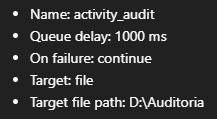
\includegraphics[width=9cm]{./Imagenes/audit1}
	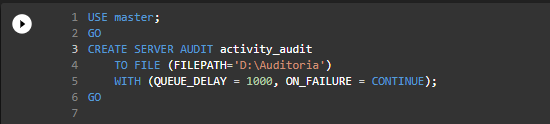
\includegraphics[width=9cm]{./Imagenes/audit2}
	\end{center}
	\end{figure}
	
	\item Paso 2: Activar la auditoria del servidor creada.

	\begin{figure}[htb]
	\begin{center}
	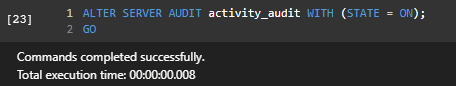
\includegraphics[width=9cm]{./Imagenes/audit3}
	\end{center}
	\end{figure}

	\item Paso 3: Crear una especificación de auditoría del servidor con las siguientes propiedades. \\\\
	\begin{figure}[htb]
	\begin{center}
	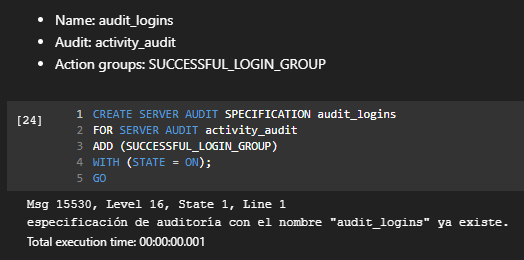
\includegraphics[width=9cm]{./Imagenes/audit4}
	\end{center}
	\end{figure}
	
	\item Paso 4: Activar la especificación de auditoria del servidor creada.\\\\\\\\
	\begin{figure}[htb]
	\begin{center}
	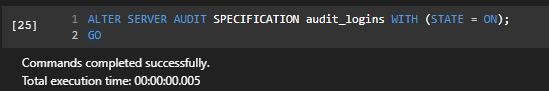
\includegraphics[width=9cm]{./Imagenes/audit5}
	\end{center}
	\end{figure}

	\item Paso 5:  Crear una especificación de auditoría de base de datos en la base de datos salesapp1 con las siguientes propiedades:
	\begin{figure}[htb]
	\begin{center}
	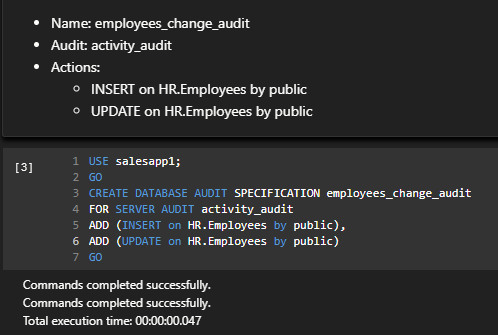
\includegraphics[width=9cm]{./Imagenes/audit6}
	\end{center}
	\end{figure}

	\item Paso 6: Activar la especificación de auditoría de base de datos creada.
	\begin{figure}[htb]
	\begin{center}
	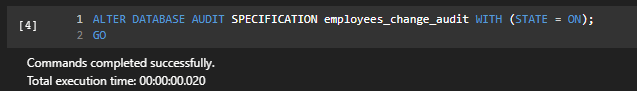
\includegraphics[width=9cm]{./Imagenes/audit7}
	\end{center}
	\end{figure}

	\item Paso 7: Ejecutar el siguiente código \\\\\\\\\\\\
	\begin{figure}[htb]
	\begin{center}
	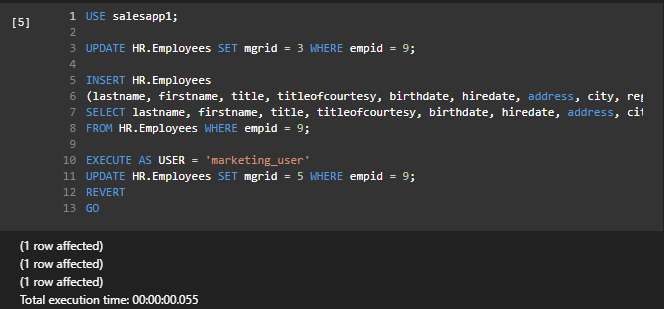
\includegraphics[width=9cm]{./Imagenes/audit8}
	\end{center}
	\end{figure}

	\item Paso 8: Escribir una consulta utilizando la función de sistema sys.fngetauditfile para devolver todos los datos de auditoría desde los archivos . 			 Filtrar los datos para que solo la actividad relacionada a la sesión actual sea visualizada. \\\\\\\\\\\\
	\begin{figure}[htb]
	\begin{center}
	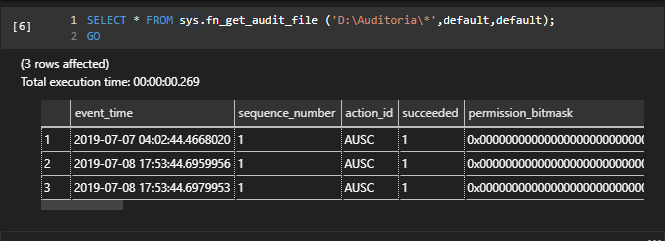
\includegraphics[width=9cm]{./Imagenes/audit9}
	\end{center}
	\end{figure}

	\item Paso 9 : Desahbilitar la auditoría de servidor activityaudit. \\\\\\\\\\\\
	\begin{figure}[htb]
	\begin{center}
	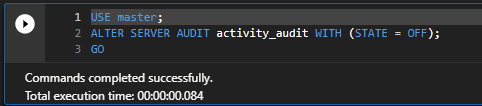
\includegraphics[width=9cm]{./Imagenes/audit10}
	\end{center}
	\end{figure}


\end{itemize}